\subsubsection{Anlehnung an Kompositionen als Vorlage eigener Werke}

\label{bkm:Ref96491192}\hypertarget{RefHeadingToc100333749}{}Neben sehr
gebräuchlichen liturgischen Formen wie Messe oder Marienlied gibt es in
Högns kirchenmusikalischem Schaffen einige Stücke mit sehr spezieller
liturgischer Funktion, wie etwa das Benedictus op. 50, die
Fronleichnams-Prozessionsgesänge op. 52, das Ecce sacerdos op. 58 und
das Juravit dominus op. 57. Nur wenige Kompositionen aus dem
Notenbestand der Ruhmannsfeldener Pfarrkirche dienen solchen
liturgischen Sonderfällen. Zu den vier oben genannten Stücken von Högn
waren deshalb nur jeweils ein oder maximal zwei entsprechende Stücke
mit derselben liturgischen Funktion von anderen Komponisten aus dem
Notenbestand aufzufinden. Die großen Gemeinsamkeiten im Aufbau, die
diese seltenen kirchenmusikalischen Stücke Högns mit ihrem Pendant aus
dem Notenbestand der Pfarrkirche aufweisen, soll im Folgenden
dargestellt werden und so Einblick in Högns Kompositionsweise erlangt
werden.

\subparagraph[Benedictus op. 50 (Deschermeier, Pilland /
Högn)]{Benedictus op. 50 (Deschermeier, Pilland / Högn)}

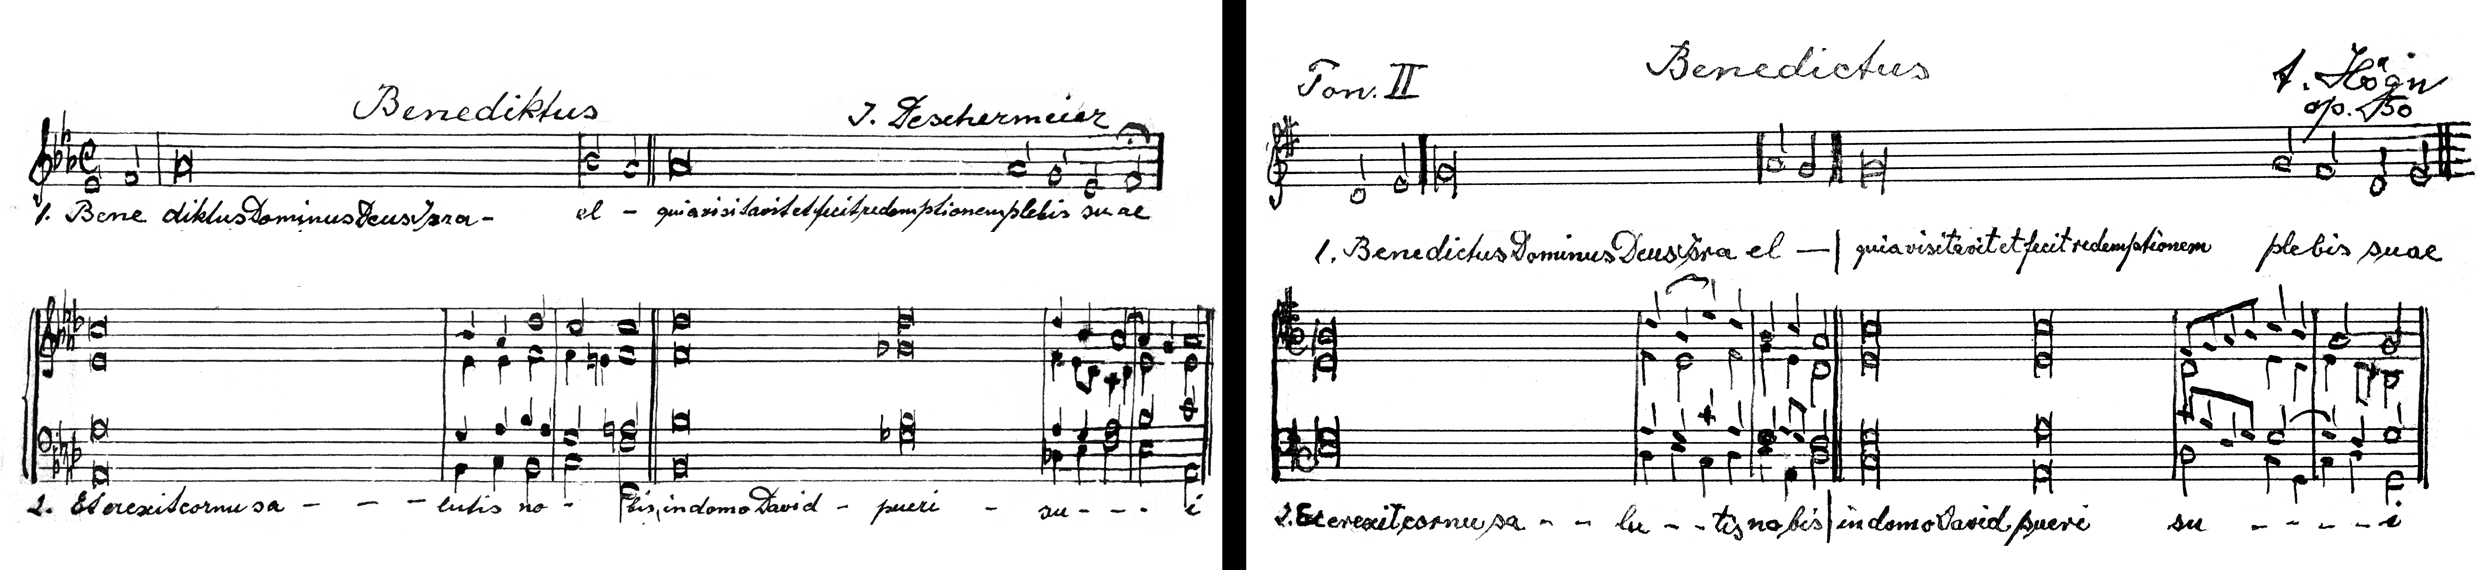
\includegraphics[width=15.977cm,height=3.671cm]{pictures/zulassungsarbeit-img080.png}


Abb. \stepcounter{Abb}{\theAbb}: Benedictus (Deschermeier / Högn)


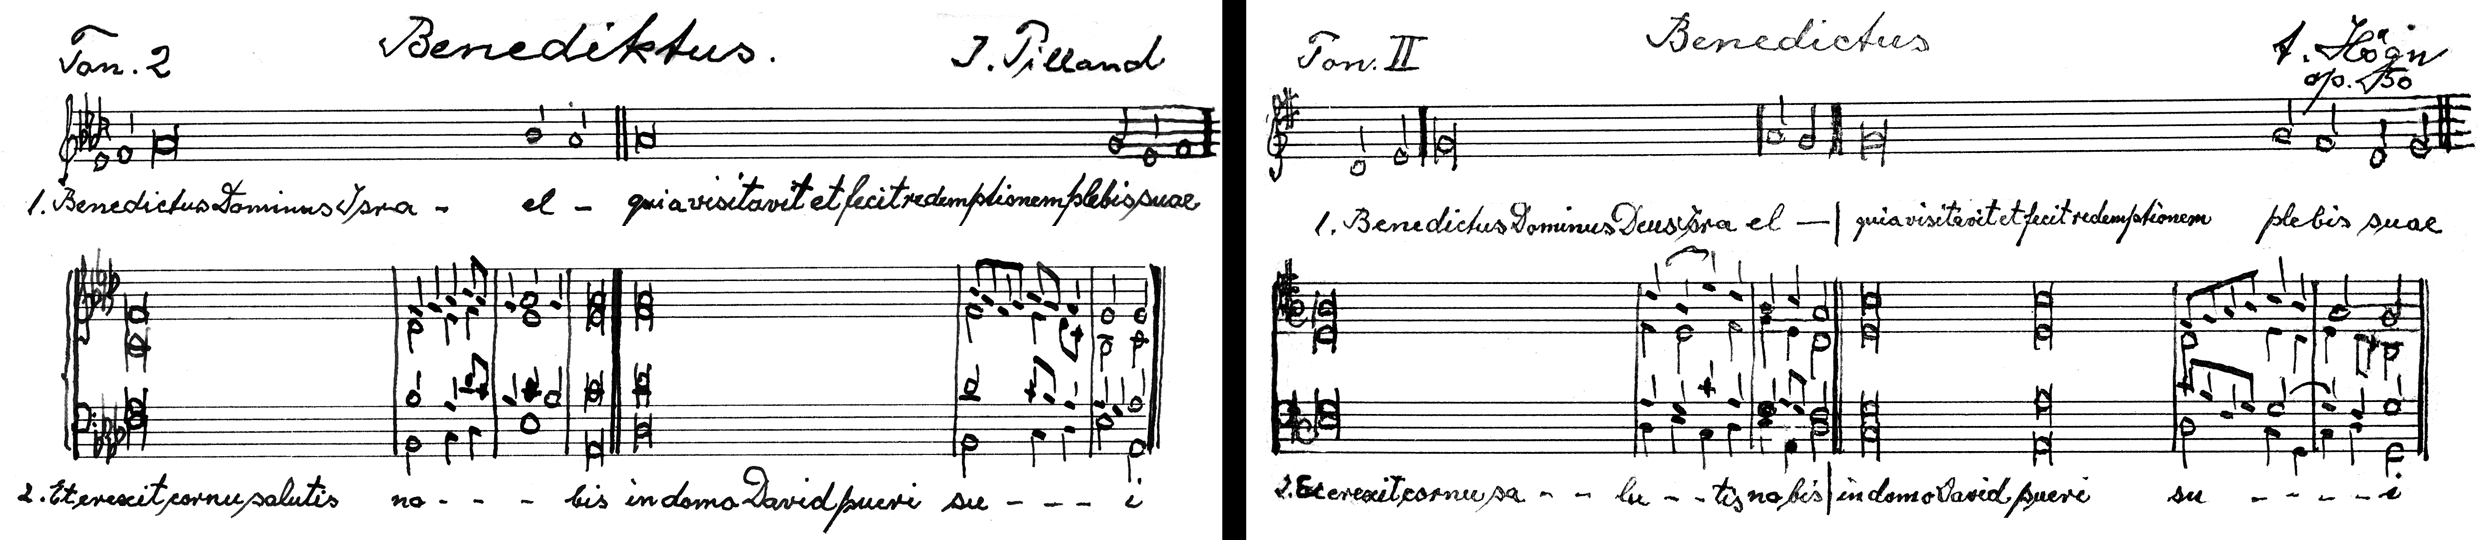
\includegraphics[width=15.977cm,height=3.478cm]{pictures/zulassungsarbeit-img081.png}


Abb. \stepcounter{Abb}{\theAbb}: Benedictus (Pilland / Högn)

Zugegebenermaßen lassen die vorliegenden Benedictus-Vertonungen,
Bestandteil der Laudes zur Osternacht, aufgrund ihrer Orientierung an
alten Formen und ihrer rezitierenden Textbehandlung wenig
kompositorischen Freiraum. So ähneln sich auch die zum Vergleich
herangezogenen Versionen von Pilland und Deschermeier (siehe Daten-CD
II). Trotzdem sind Übereinstimmungen im Aufbau in beiden Stücken mit
Högns Komposition zu erkennen. Die Schreibart der ersten Choralzeile
hat Högn von Deschermeier übernommen, ebenso die Aufteilung des
Haltetons in der zweiten Hälfte der zweiten Choralzeile auf zwei
Akkorde und die Textverteilung. Högn und Deschermeier verlassen den
ersten Halteton der zweiten Choralzeile schon auf der zweiten Silbe von
„salutis“, während hingegen Pilland nur das Wort „nobis“ melismatisch
vertont und „salutis“ noch syllabisch behandelt. Wenn man als
Grundtonart die in der letzten Kadenz vorherrschende Tonart annimmt,
beginnen Pilland und Högn die zweite Choralzeile mit dem Akkord der VI.
Stufe. Högn setzt diesen Akkord aber in Quintstellung und legt so am
Übergang von erster zur zweiten Choralzeile die Stimmführung im Sopran
in Analogie zur Version von Deschermeier an. Das Motiv, das die ersten
vier Töne im vorletzten Takt im Sopran der Komposition von Pilland
bilden, tritt bei Högn an entsprechender Stelle im Tenor in nur
geringfügig veränderter Form auf. Bei dem Stück Benedictus op. 50 kann
Högn nur eine sehr geringe kompositorische Eigenleistung zuerkannt
werden. Einige Wendungen aus Deschermeiers und Pillands Kompositionen
zitiert Högn exakt. Die übrigen Stellen in Högns Stück wirken eher als
Variation oder Abwandlung der entsprechenden Stellen in den Werken von
Deschermeier und Pilland als eigenständige musikalische Gedanken.

\subparagraph{Fronleichnams-Prozessionsgesänge op. 52 (Goller / Högn)}
Schon der gleich lautende Titel „Prozessionsgesänge für das hochheilige
Fronleichnamsfest“ der Kompositionen von Vinzenz Goller und August Högn
deutet darauf hin, dass Högn sein op. 52 in Anlehnung an das op. 32 von
Goller (siehe Daten-CD II) komponiert hat. Eine Reihe von weiteren
Übereinstimmungen der beiden Prozessionsgesänge im Aufbau und in der
Textbehandlung lassen keinen Zweifel aufkommen, dass Högn beim
Komponieren seiner Prozessionsgesänge das entsprechende Werk von Goller
als Vorlage benutzt hat. Die Prozessionsgesänge setzen sich bei beiden
Komponisten aus jeweils 14 einzelnen Stücken zusammen. Vor allem die
Übereinstimmung derjenigen Stücke, die bei Goller und Högn in der
Abfolge der Gesänge dieselbe Position einnehmen und deshalb auch
denselben Text und Titel verwenden, soll im Folgenden bestätigt werden.
Wörtlich übernimmt Högn sämtliche Untertitel zu den 14 einzelnen
Stücken aus Gollers Prozessionsgesängen wie etwa „Auf dem Wege von der
Kirche zum I. Altare.“ Es liegt an der Textaufteilung auf die
Gesangsstimmen, die Högn exakt von Goller kopiert, dass sowohl Taktart
als auch die Anzahl der Takte der Chorpassagen bei den meisten
entsprechenden Stücken der beiden Kompositionen genau übereinstimmen.
Die Anzahl der Takte des Vorspiels ist zwar nur bei fünf
korrespondierenden Stücken genau gleich, doch bei den meisten
entsprechenden Stücken, die eine unterschiedliche Taktanzahl im
Instrumentalvorspiel haben, weicht die Anzahl der Takte jeweils nur um
einen Takt voneinander ab. Bei vier entsprechenden Stücken bringt Högn
anders als Goller Nachspiele an. Die vergleichbaren Stücke, die in
Gollers Version ein Nachspiel haben, enden auch bei Högn mit einem
Nachspiel. Bei mehr als der Hälfe der korrespondierenden Stücke mit
einem „Amen“ als Textabschluss ist die Anzahl der Takte, die zur
Vertonung des „Amens“ benötigt werden, bei beiden Komponisten gleich.
Die folgende Tabelle soll die Übereinstimmungen beziehungsweise
Abweichungen der einzelnen entsprechenden Stücke von beiden
Prozessionsgesängen anführen. Als Abkürzungen werden verwendet:
Vorspiel = Anzahl der Takte des Instrumentalvorspiels; Text = Anzahl
der Takte der Textvertonung ohne „Amen“; Amen = Anzahl der Takte der
Amen-Vertonung; Nachspiel = Anzahl der Takte des
Instrumentalnachspiels; „/“ = links vom Schrägstrich werden Merkmale
von Gollers Komposition aufgeführt, rechts Merkmale von Högns
Kompositionen (Goller/Högn); „-“ = kein Vor-, Nachspiel oder
Amen-Vertonung vorhanden; Dunkelgrau markierte Zellen = große
Abweichung; Hellgrau markierte Zellen = geringe Abweichung; Zellen ohne
Markierung = exakte Übereinstimmung.

{\centering   [Warning: Image ignored]
% Unhandled or unsupported graphics:
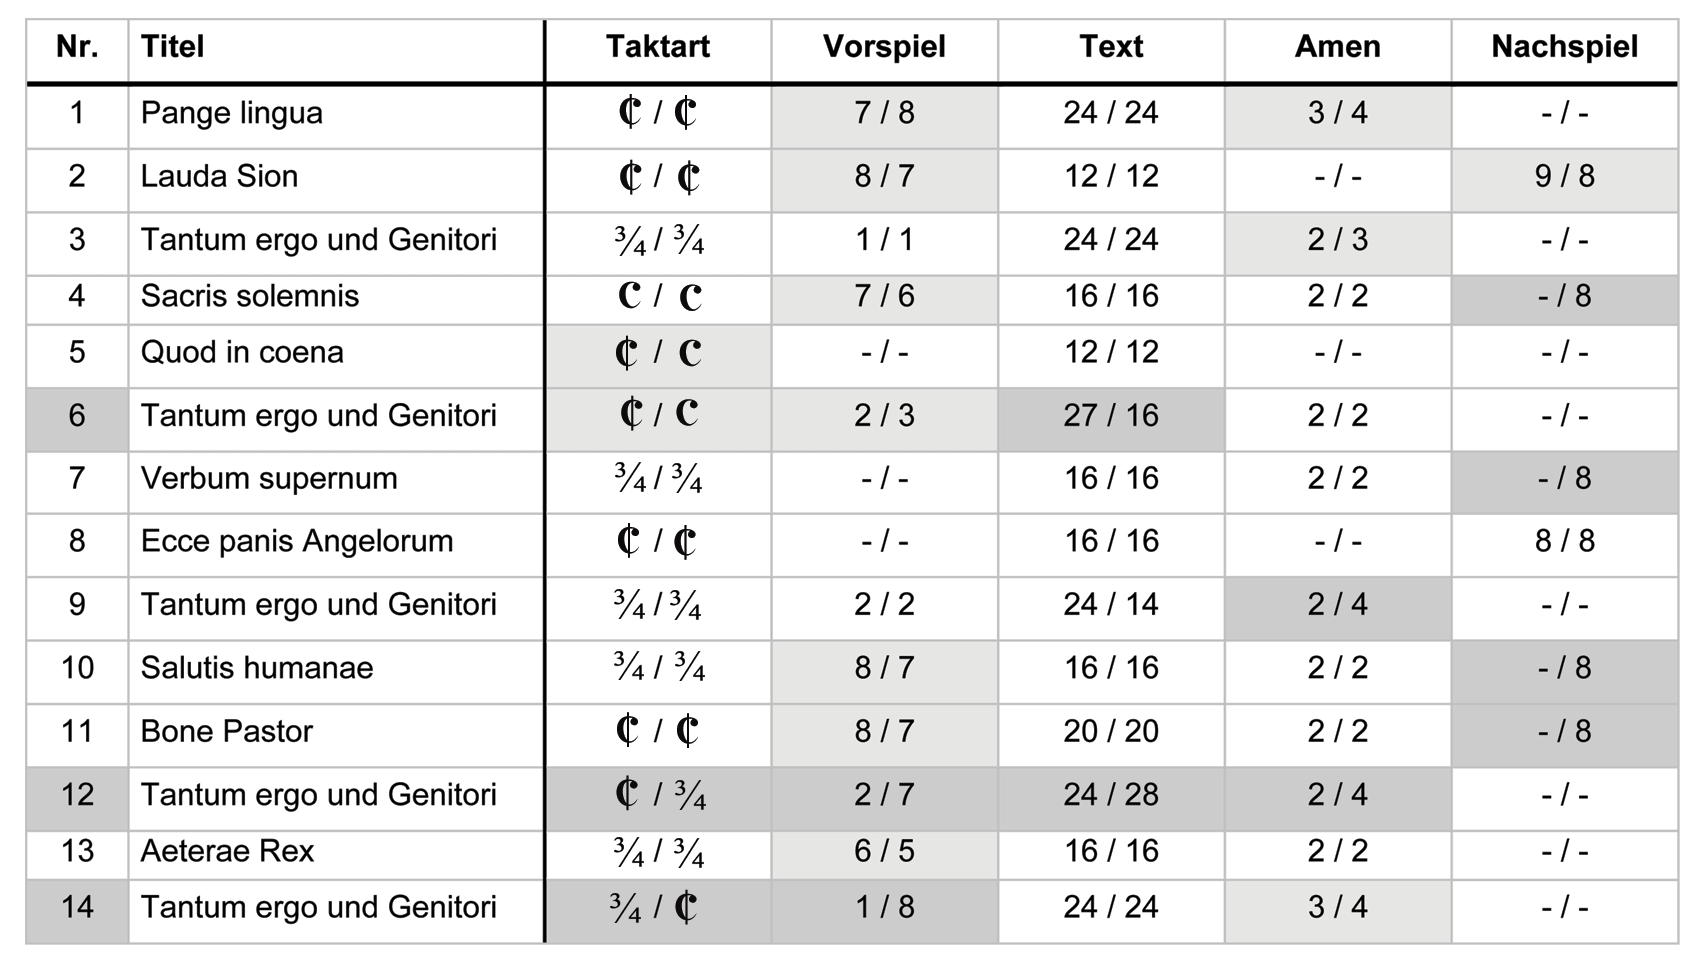
\includegraphics[width=13.088cm,height=7.486cm]{pictures/zulassungsarbeit-img082.png}
 \par}
Nur drei Stücke aus Högns Prozessionsgesängen, nämlich die Nr. 6, 12 und
14, wie der Tabelle zu entnehmen ist, unterscheiden sich deutlich von
den entsprechenden Stücken aus Gollers Prozessionsgesängen bezüglich
Textbehandlung und Aufbau. Dass sich Högn bei den eben genannten
Stücken keine entsprechende Stücke von Goller zum Vorbild nimmt, liegt
weniger an einer anderen Kompositionsweise, die bei diesen Stücken
anwandte, sondern an Maßnahmen, die ihm das Komponieren dieser Stücke
ersparten. Die Nr. 14 ist in Högns Werk nicht ausnotiert, Es wird
lediglich auf die Nr. 1 verwiesen. Das ist möglich, da das erste Stück,
ein Pange lingua, auch die für das letzte Stück benötigten Strophen
„Tantum ergo Sacramentum …“ und „Genitori, Genitoque …“ enthält.
Gollers Gesänge enthalten als Schlussstück ein eigenständiges Stück.
Högns Nr. 6 in den Prozessionsgesängen entspricht seinem Pange lingua
F-Dur op. 43. Högn hat also ein früheres Werk in den
Prozessionsgesängen aufgenommen. Beim 12. Stück in den
Prozessionsgesängen handelt es wieder um die häufig vorkommende
liturgische Form eines Tantum ergos. Es ist wahrscheinlich, dass Högn
bei der Nr. 12 ähnlich wie bei der Nr. 6 vorgegangen ist und eine
frühere Komposition übernommen hat, die aber als eigenständiges Werk
nicht überliefert ist.

Ein Vergleich der Stücke Nr. 8 und Nr. 10 aus den Prozessionsgesängen
beider Komponisten soll exemplarisch die oben angeführten
Übereinstimmungen der entsprechenden Stücke verdeutlichen und darüber
hinaus Ähnlichkeiten im verwendeten motivischen Material zwischen den
Stücken Nr. 8 und Nr. 10 von Goller und Högn nachweisen.


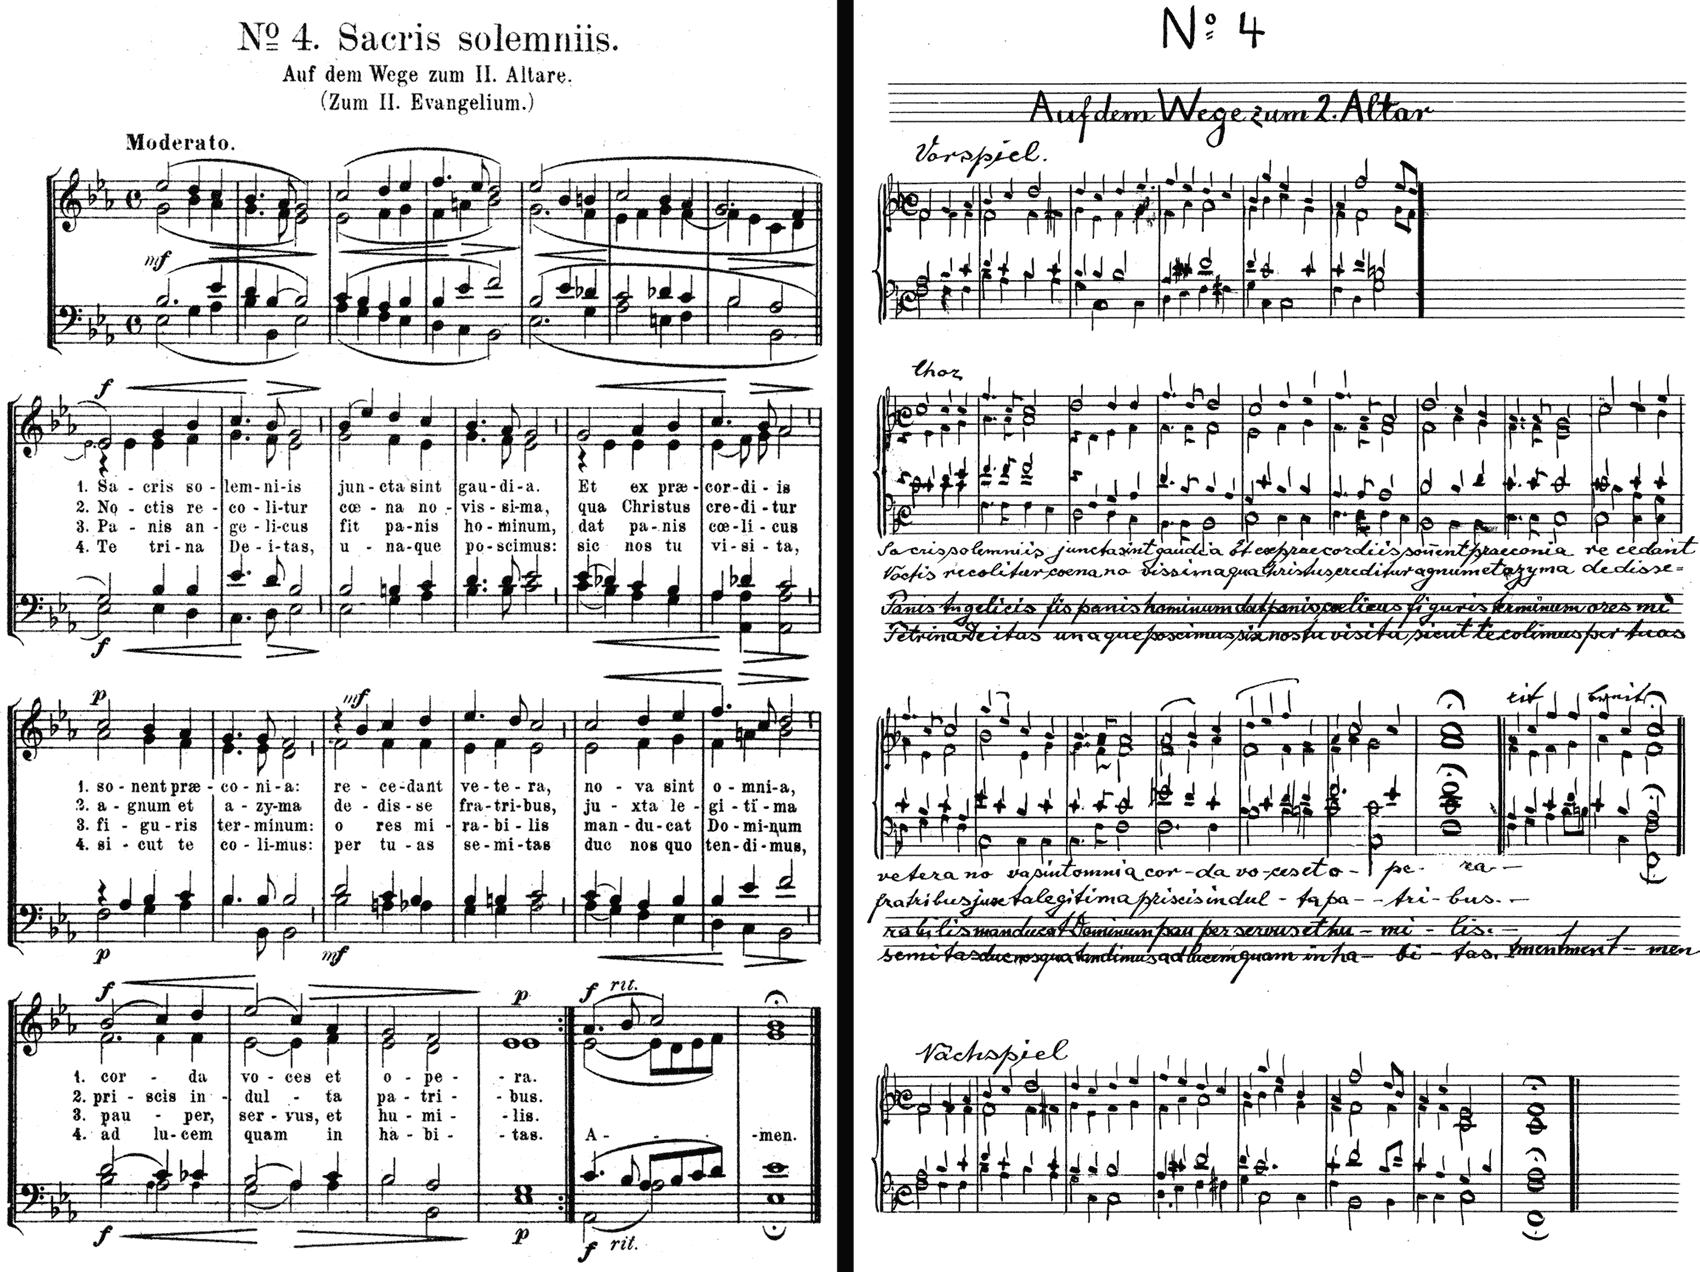
\includegraphics[width=15.967cm,height=11.947cm]{pictures/zulassungsarbeit-img083.png}


Abb. \stepcounter{Abb}{\theAbb}: Fronleichnams-Prozessionsgesänge, Nr. 4
(Goller / Högn)

Die Nr. 4 mit dem Titel „Sacris solemniis“ ist eines der wenigen Stücke
aus Gollers Fronleichnams-Prozessionsgesängen mit charakteristischer
Rhythmik. Eine prägnante Punktierung unterstützt die Betonung zur Mitte
der zweitaktigen Phrasen. Högn übernimmt nicht nur rhythmisch diese
Phrasierung, sondern verdeutlicht auch wie Goller den Schwerpunkt in
der Phrase durch eine zur Phrasenmitten ansteigende und dann
absteigende Melodieführung. Beide verlassen dieses Schema der
zweitaktigen Auf- und Abbewegung der Sopranstimme nach 6 Takten – vom
Choreinsatz aus gesehen – durch Verwendung einer absteigenden Linie.
Die letzten 4 Takte einer Strophe gestaltet Högn in Analogie zu Gollers
„Sacris solemniis“ in einer viertaktigen Phrase, wobei hier ebenfalls
wie bei Goller die Punktierung wegfällt. Auch ein Detail scheint Högn
bei Goller entlehnt zu haben, nämlich die bei Phrasenbeginn um eine
Zählzeit verzögerten Stimmeinsätze in den Takten 8, 12, 14 und 16 bei
Goller. Den Effekt, dass eine Stimme zu Phrasenbeginn eine Zählzeit
später einsetzt, setzt Goller regelmäßig im ganzen Chorteil in
verschiedenen Stimmen ein. Högn dagegen wendet diesen Effekt nur in
seinen ersten beiden Phrasen in den Mittelstimmen an (Takt 7 und 9) und
verursacht somit eine gewisse Asymmetrie im Satzbild.


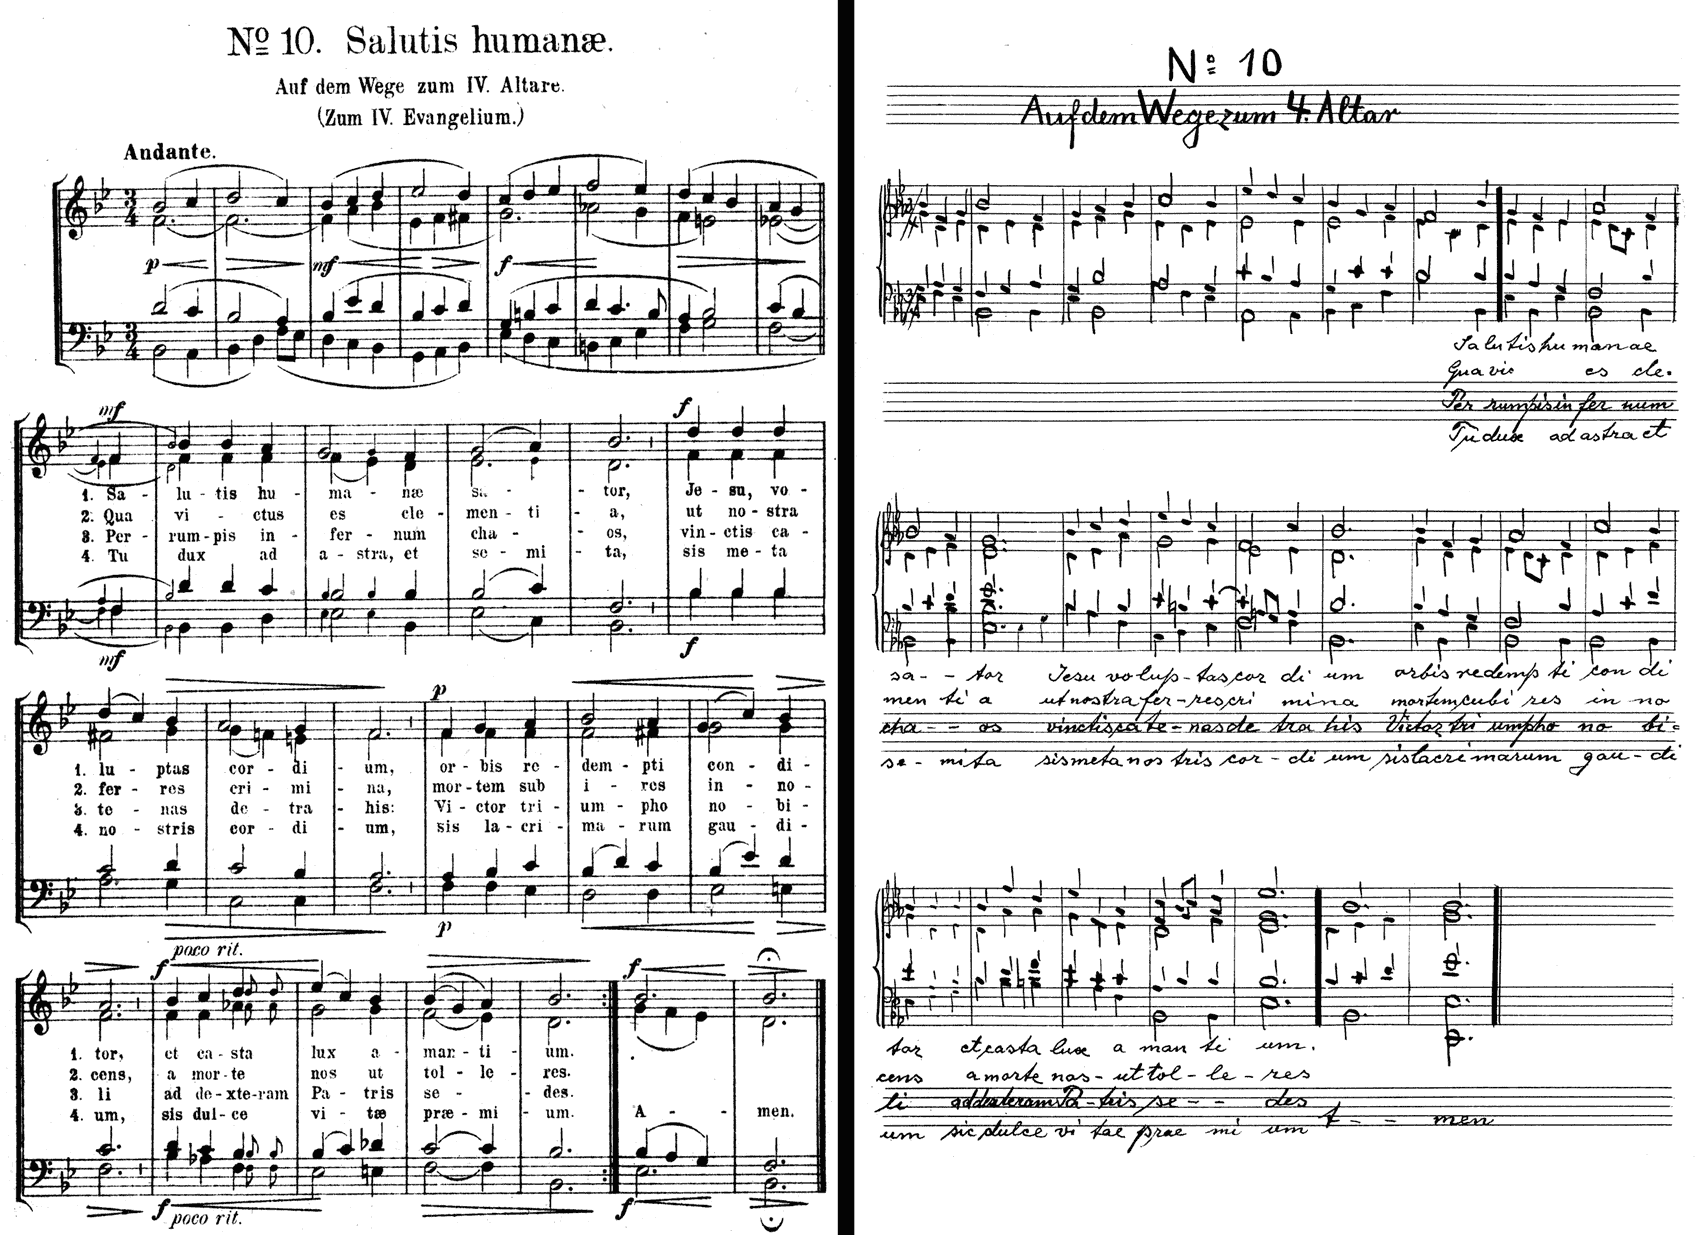
\includegraphics[width=15.967cm,height=11.599cm]{pictures/zulassungsarbeit-img084.png}


Abb. \stepcounter{Abb}{\theAbb}: Fronleichnams-Prozessionsgesänge, Nr.
10 (Goller / Högn)

Die natürliche Wortbetonung der Textvorlage zu der Nr. 10 der
Prozessionsgesänge legt eine Vertonung mit Auftakt im ¾-Takt nahe
(Salûtis humânae satôr). Doch man kann den Text auch anders umsetzen,
wie an Hallers ganztaktig beginnender Vertonung aus den „Laudes
Eucharesticae“ zu sehen ist, die ebenfalls von Högn nachweislich an
Fronleichnam zur Aufführung gebracht wurden. So dürfte der Choreinsatz
in Högns Komposition von Goller beeinflusst worden sein, zumal der
Beginn des Gesangs nicht nur wie Gollers Choreinsatz mit einem Auftakt
beginnt, sondern der Einsatz des Chores auch noch an der überleitenden
Kadenz des Instrumentalvorspiels mit Takterstickung beteiligt ist. Zwar
führt Högn die Melodiestimme des Soprans in seiner Nr. 10 viel
sprunghafter in Vergleich zu Gollers Oberstimmenbewegung, doch die
entsprechenden Phrasen beider Kompositionen bedienen sich derselben
Registerlage der Sopranstimme. Högn wie Goller überschreiten in der 1.
und 3. Textzeile das b’ im Sopran fast nie, gehen aber in der 2. und 4.
Zeile deutlich darüber hinaus. Unverkennbar hatte die Floskel der
Mittelstimmen aus Högns „Amen“-Vertonung ihr Vorbild im Schluss von
Gollers Komposition, auch wenn die Viertelbewegung bei Högn in eine
andere Richtung weist.

Würden auch die Stücke mit den Nummern 6, 12 und 14 in Högns
Prozessionsgesängen ähnlich große Übereinstimmungen mit den
entsprechenden Stücken aus Gollers Prozessionsgesängen zeigen, wie die
übrigen Stücke aus Högns op. 52, wäre Högns Komposition ein
Paradebeispiel für ein Plagiat.

\subparagraph[Ecce sacerdos op. 57 (Kempf / Högn)]{Ecce sacerdos op. 57
(Kempf / Högn)}
Derselbe Untertitel „zum feierlichen Empfang eines Bischofs“ und die
gleiche Tempoangabe „Maestoso“ deuten an, dass Högn das Ecce sacerdos
As-Dur op. 12 von Richard Kempf als Kompositionsvorlage zu seinem Ecce
sacerdos F-Dur op. 57 (siehe auch Daten-CD II) diente. Jeden Zweifel,
dass Högn sein Ecce sacerdos vielleicht doch ohne Vorlage komponiert
haben könnte, beseitigt Högns Zitat des nach unten gerichteten
Tonleiterausschnitts vom Grundton zur Quarte der Orgel im Takt 1 von
Kempfs Ecce sacerdos.


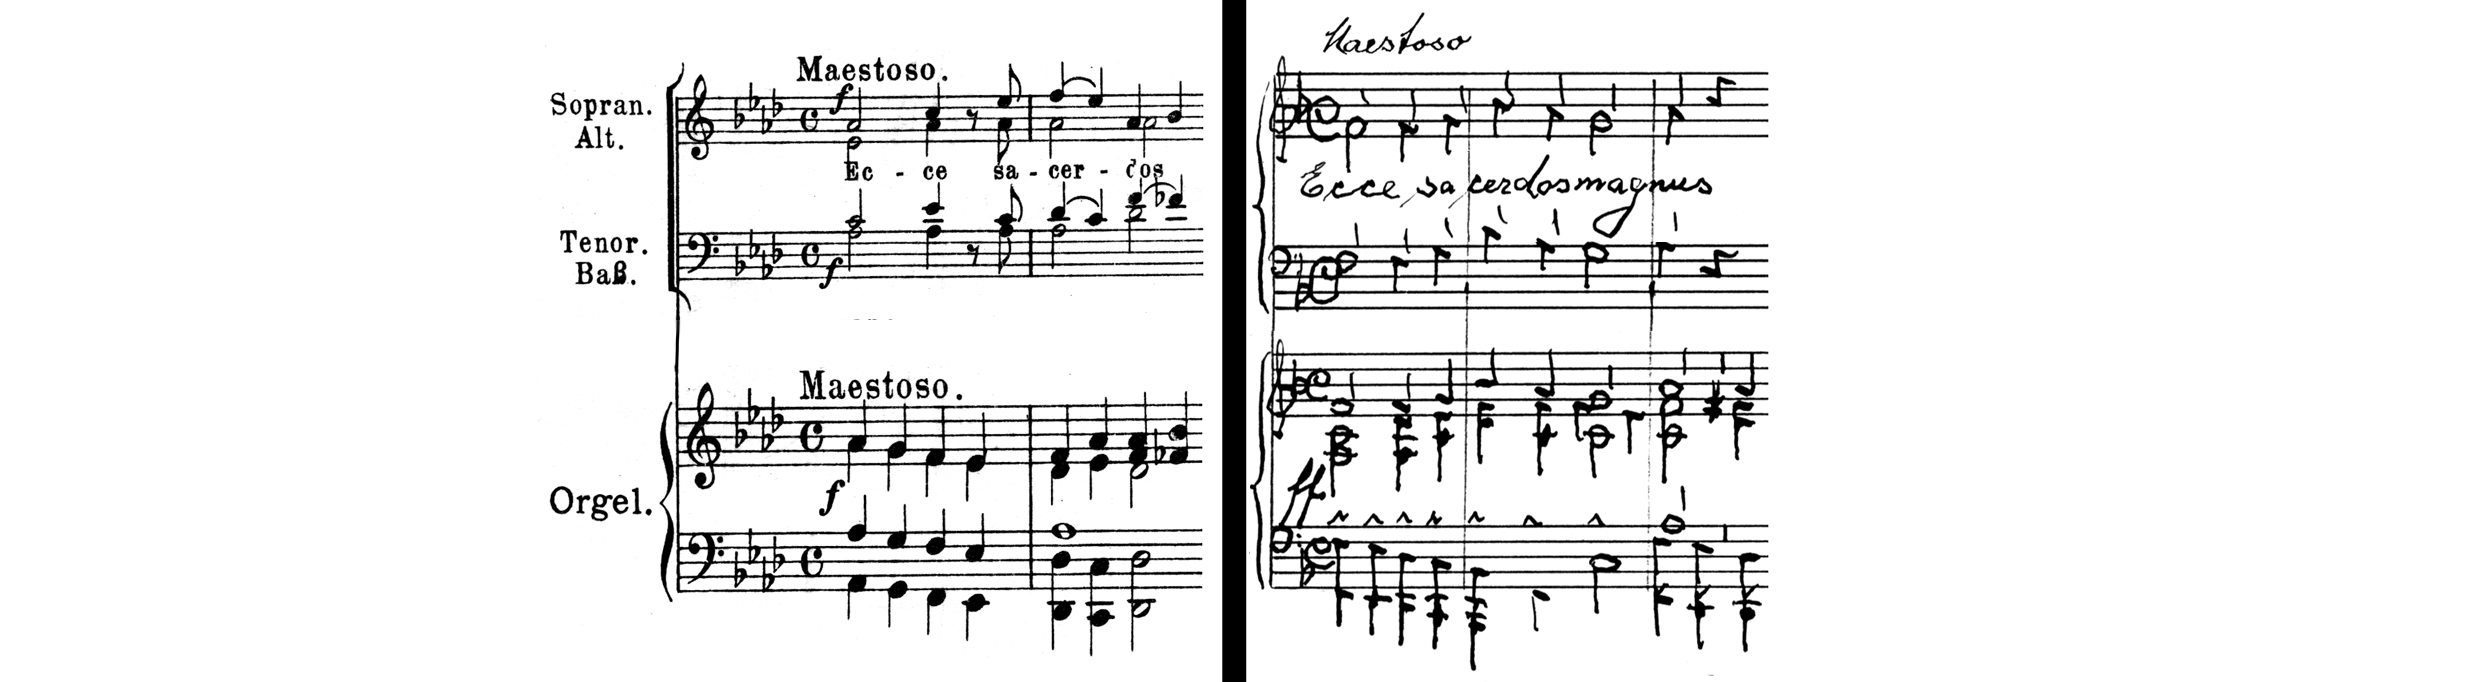
\includegraphics[width=15.977cm,height=4.394cm]{pictures/zulassungsarbeit-img085.png}


Abb. \stepcounter{Abb}{\theAbb}: Ecce sacerdos (Kempf / Högn), Takt 1 –
2  / Takt 1 – 3

Übereinstimmungen sind auch bei den beiden Vertonungen der Textpassage
„qui in diebus suis placuit Deo“ zu erkennen. Im Unterschied zu Kempf
behandelt Högn die Stelle zwar homophon, aber er verwendet dabei im
Sopran eine Melodieführung, die dem Rhythmus und der Bewegungsrichtung
des Motivs, das Kempf zur Imitation verwendet, entspricht. Ein
Vergleich der Sopranstimmen bei Kempf in den Takten 14 bis 17 und bei
Högn in den Takten 7 bis 10, ergibt, dass neben der rhythmischen
Übereinstimmung und der Bewegungsrichtung der Abstand zwischen
Anfangston und Endton bei beiden Stimmen jeweils eine Quarte beträgt.


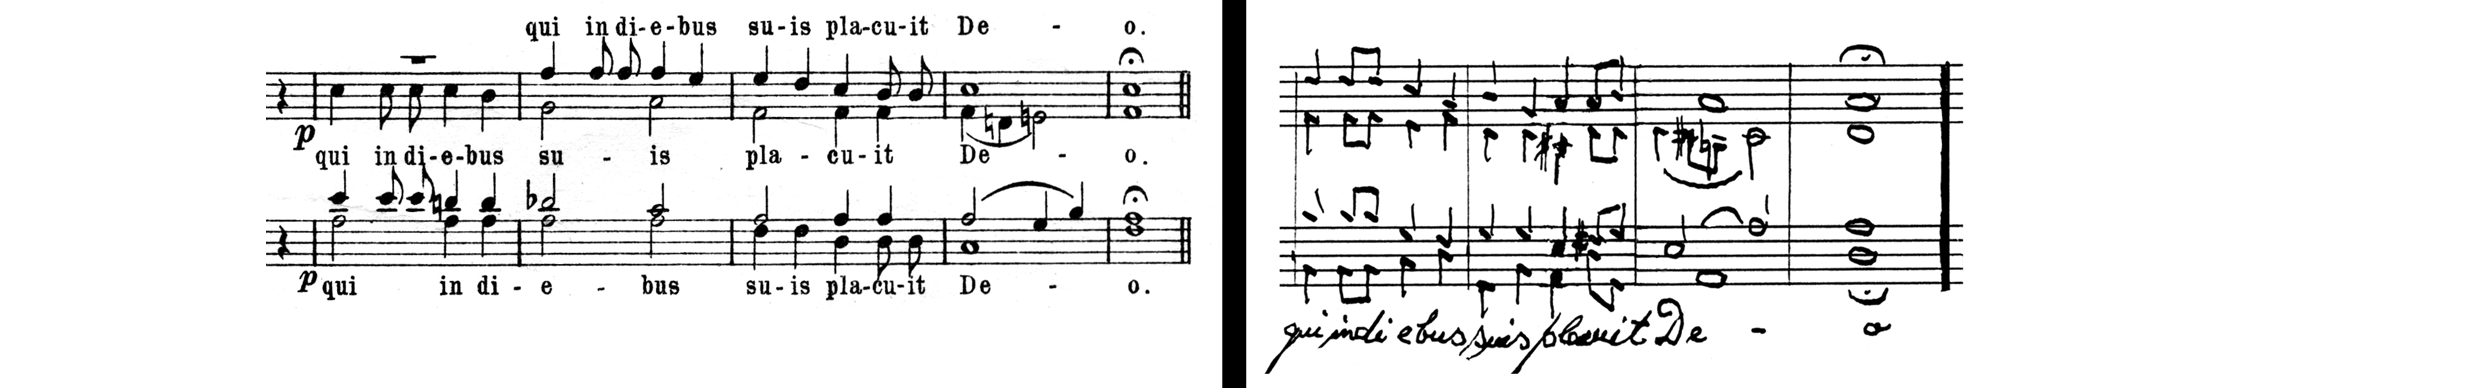
\includegraphics[width=15.977cm,height=2.499cm]{pictures/zulassungsarbeit-img086.png}


Abb. \stepcounter{Abb}{\theAbb}: Ecce sacerdos (Kempf / Högn), Takt 13 –
17 / Takt 7 – 10

Obwohl Högns 12 Takte umfassende Vertonung der Textzeile „Ideo jure
jurando fecit illum Dominus crescere in plebem suam” um 4 Takte kürzer
ist als die entsprechende Passage bei Kempf, ist eine Orientierung von
Högn an seiner Kompositionsvorlage auch in diesem Abschnitt
unverkennbar. Beide Komponisten gestalten den Chorpart zu Beginn dieses
Abschnitts (Kempf Takt 18, 19/ Högn Takt 11 12) im Unisono und im
selben Rhythmus. Nach der Unisono-Stelle folgen bei beiden
Kompositionen zwei imitatorische Teile mit jeweils einem Motiv. Hat
Högns Motiv zur Vertonung des Textes „fecit illum Dominus“ in seiner
Linearität Ähnlichkeit mit Kempfs Motiv an entsprechender Stelle, wählt
Högn zur Unterlegung des Textes „crescere in plebem suam” ein
vollkommen anderes Tonmaterial als Kempf und büßt so ein gewisses Maß
an nachvollziehbarer Textausdeutung ein. Indem Högn nicht wie Kempf
Stimmeinsätze von unten nach oben und ein nach oben gerichtetes Motiv
wählt, sondern geradezu die gegenteiligen Mittel wählt, nämlich
Stimmeinsätze von oben nach unten und ein nach unten gerichtes Motiv,
bei dem aufgrund seiner Punktierung der abwärtsstrebenen Charakter noch
verstärkt wahrgenommen wird, kann von einer sinngerechten Vertonung des
Wortes „crescere” also „wachsen” bei Högn keine Rede sein.


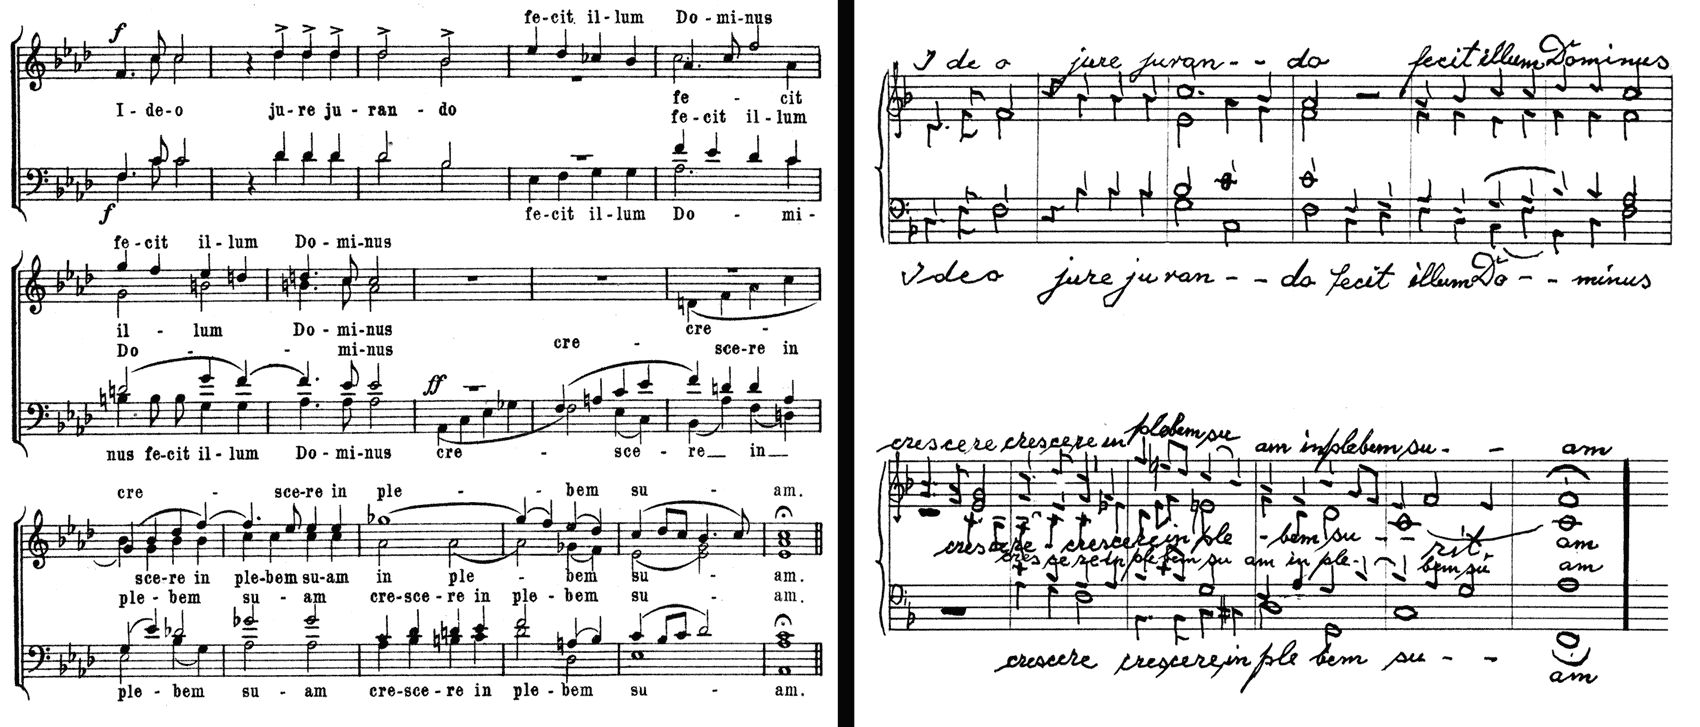
\includegraphics[width=15.967cm,height=6.828cm]{pictures/zulassungsarbeit-img087.png}


Abb. \stepcounter{Abb}{\theAbb}: Ecce sacerdos (Kempf / Högn), Takt 18 –
 33 / Takt 11 –  22

Nicht nur in der Wahl der Motive und der Gestaltung einzelner Abschnitte
gibt es bei Högn Übereinstimmungen zu der Komposition von Kempf,
sondern auch im großformalen Aufbau. Ähnlich wie Kempf vertont Högn
jeden Satz der Textvorlage (siehe unten) in einem eigenen,
abgeschlossenen musikalischen Abschnitt. Die Anordnung der einzelnen
Abschnitte, am auffälligsten die dreimalige Wiederholung der Textzeile
„Ideo jure jurando …“, ist ebenfalls bei beiden Kompositionen
identisch.

Ecce sacerdos magnus, qui in diebus suis placuit Deo.

Ideo jure jurando fecit illum Dominus crescere in plebem suam.

Benedictionem omnium gentium dedit illi et testamentum suum confirmavit
super caput eius.

Ideo jure jurando fecit illum Dominus crescere in plebem suam.

Gloria Patri et filio et Spiritui sancto.

Ideo jure jurando fecit illum Dominus crescere in plebem suam.

(Auszug aus Ecc. 44, 16-27; 45, 3-20)

Da Högn bei seinem Ecce sacerdos durchaus eigene Lösungen findet,
beispiels-weise in der Vertonung der Textzeile „Benedictionem omnium
…“, triff die Bezeich-nung Plagiat bei dieser Komposition nicht zu. Der
große Einfluss von Kempfs Ecce sacerdos ist aber anderseits auch nicht
zu übersehen.

\clearpage\subparagraph{Juravit Dominus op. 58 (Alt / Högn)}
Um nicht den Eindruck zu hinterlassen, dass Högn nur Plagiate erstellte,
sei an dieser Stelle ein Vergleich zwischen dem Juravit Dominus op. 19
von G. M. Alt und dem Juravit Dominus op. 58 von Högn (siehe Daten-CD
II) angebraucht. Alts Werk diente Högn nur als Textvorlage, wie auch
schon beim Vergleich der beiden Titelblätter zu sehen ist, nicht als
Vorlage zur musikalischen Umsetzung des Textes.


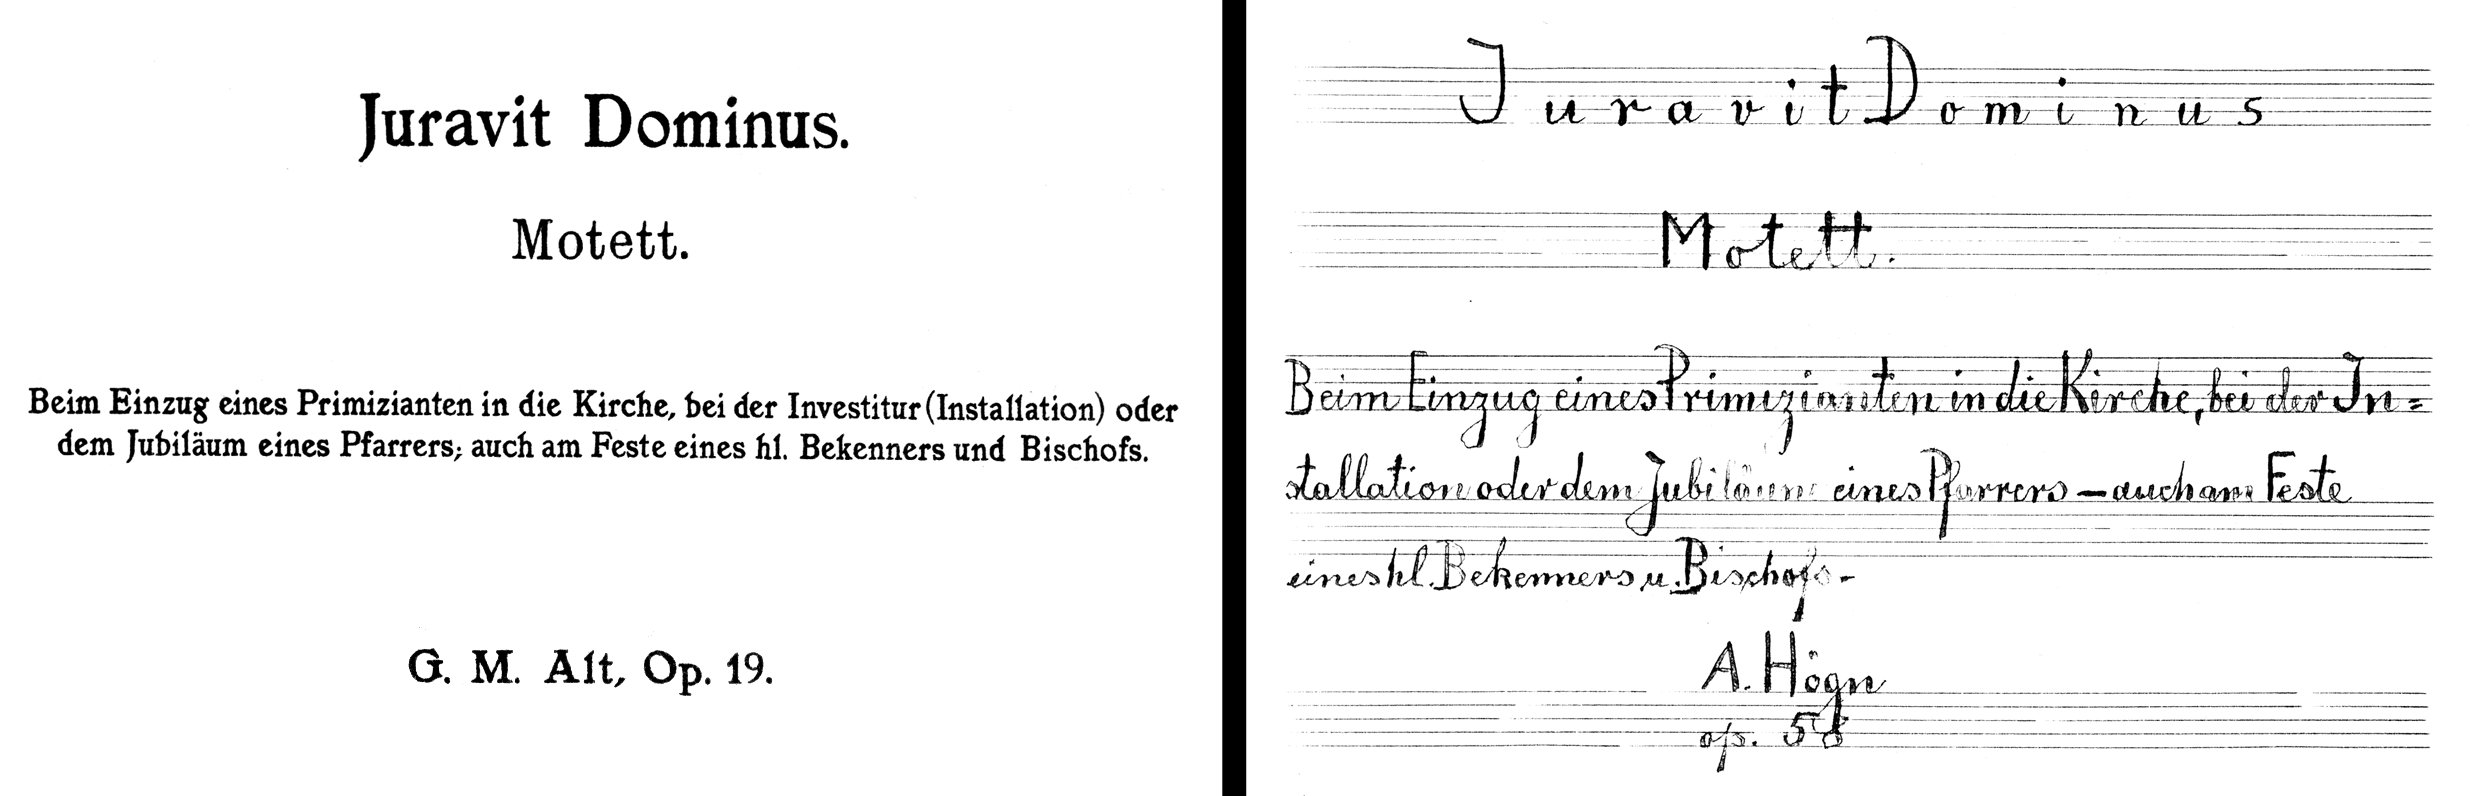
\includegraphics[width=15.977cm,height=5.128cm]{pictures/zulassungsarbeit-img088.png}


Abb. \stepcounter{Abb}{\theAbb}: Juravit Dominus (Alt / Högn),
Titelblatt

Im musikalischen Aufbau knüpft das Juravit Dominus op. 58 eher an Högns
letzte Komposition, an das Ecce sacerdos op. 57, als an Alts
Kompositionen an. Das Juravit dominus von Högn zeichnet sich durch eine
Imitation zwischen Chor und Bläserquartett mit einem auftaktigen Motiv
aus, das den Bläsereinwürfen im Ecce sacerdos entlehnt ist. Es entsteht
eine kunstvolle Doppelchörigkeit, die um einiges origineller wirkt, als
der homophone, auf Kadenzharmonik beruhende und deshalb plump wirkende
Satz bei Alt. Da Högn bei seinem Juravit Dominus musikalisch einen
vollkommen eigenständigen Weg einschlägt, verwundert es schon, wenn er
trotzdem Alts Textverteilung fast eins zu eins übernimmt (siehe unten).
So wird wie bei Alt die erste Textzeile „Juravit Dominus, et non
poenitebit eum“ dreimal wiederholt, die erste Hälfte der zweiten
Textzeile „Tu es sacerdos in aeternum“ ebenfalls dreimal und der
Schluss der zweiten Textzeile „secundem ordinem Melchisedech“ nur
zweimal. Dass Högn einmal zusätzlich die Wörter „secundem ordinem“
wiederholt, ändert an der grundsätzlichen Übereinstimmung in der
Textverteilung wenig.

Juravit Dominus, et non poenitebit eum.

Juravit Dominus, et non poenitebit eum.

Juravit Dominus, et non poenitebit eum.

Tu es sacerdos in aeternum,

Tu es sacerdos in aeternum,

Tu es sacerdos in aeternum,

secundem ordinem (secundem ordinem) Melchisedech,

secundem ordinem Melchisedech.

(Psalm 109,4)

Offenbar hat Högn an seiner sehr einfach strukturierten Vorlage wenig
Gefallen gefunden und deshalb auf eine Übernahme von musikalischem
Material aus Alts Juravit Dominus verzichtet.

Es wäre durchaus denkbar, dass Högn nicht nur bei diesen oben
dargestellten vier liturgischen Sonderfällen ein bestimmtes Werk zum
Vorbild nahm, sondern auch bei gebräuchlicheren Formen, wie etwa
Messen, Marienliedern oder Grabliedern, nur ist wegen Fülle an Material
im Notenbestand der Ruhmannsfeldener Kirche der Nachweis hier weitaus
schwieriger zu führen, als bei speziellen Formen, die meist Unikate im
Notenbestand sind. Tatsächlich lassen sich in den meisten Kompositionen
von Högn Elemente eines Personalstils aufzeigen.